\section{Grammar-based Whitebox Fuzzing Using Symbolic Execution}
\subsection{Whitebox Fuzzing}
Whitebox fuzzing~\cite{fuzzing} executes the program under test with an initial, well-structured input, both concretely and symbolically. Along the execution, symbolic execution collects constraints on program inputs from the predicates in the conditional statements. The conjunction of these constraints of a execution path form an expression, called path condition. Satisfying the negation of each constraint in the path condition defines new inputs that exercise different control paths. Whitebox fuzzing repeats this process for the newly created inputs, with the goal of exercising many different control paths of the program under test and finding defects as fast as possible using various search heuristics. In practice, the search is usually incomplete because the number of feasible control paths grows exponentially with number of conditional statements in the program under test and because the precision of symbolic execution, constraint generation and solving is inherently limited. However, whitebox fuzzing has been shown to be very effective in finding new security vulnerabilities in several applications.

In practice, the current effectiveness of whitebox fuzzing is limited when testing applications with highly structured
inputs, e.g., compilers and interpreters. These applications process their inputs in stages, such as lexing, parsing and evaluation. Because of the enormous number of control paths in early processing stages, whitebox fuzzing rarely reaches parts of the application beyond these first stages. For instance, there are many possible sequences of blank-spaces/tabs/carriagereturns/etc. separating tokens in most structured languages, each corresponding to a different control path in the lexer. In addition to path explosion, symbolic execution may fail already in the first processing stages. For instance, lexers often detect language keywords by comparing their pre-computed, hard-coded hash values with the hash values of strings read from the input; this effectively prevents symbolic execution and constraint solving from ever generating input strings that match those keywords, since hash functions cannot be inversed (i.e., given a constraint x == hash(y) and a value for x, one cannot compute a value for y that satisfies this constraint).

In \cite{grammar}, Godefroid et al. propose a new approach, called \textit{grammar-based whitebox fuzzing}, which enhances whitebox fuzzing with a grammar-based specification of valid inputs. They present a dynamic test generation algorithm where symbolic execution directly generates grammar-based constraints whose satisfiability is checked using a custom grammar-based constraint solver. Their algorithm consists of two key components:

\begin{enumerate}
\item Generation of higher-level symbolic constraints, expressed in terms of symbolic grammar tokens returned by the
lexer, instead of the traditional~\cite{dart,exe,fuzzing} symbolic bytes read as input.
	
\item A custom constraint solver that solves constraints on symbolic grammar tokens. The solver looks for solutions
that satisfy the constraints and are accepted by a given (context-free) grammar.
\end{enumerate}

\subsection{Example}
Their algorithm never generates non-parsable inputs, i.e., the inputs generates can be accepted by the lexer and parser. In addition, the grammar-based constraint solver can complete a partial set of token constraints into a fully-defined valid input, thus avoiding exploring many possible non-parsable paths. By restricting the search space to parsable inputs, grammar-based whitebox fuzzing can explore deeper paths, and focus the search on the harder-to-test, deeper processing stages.


\begin{figure}[h]
\centering
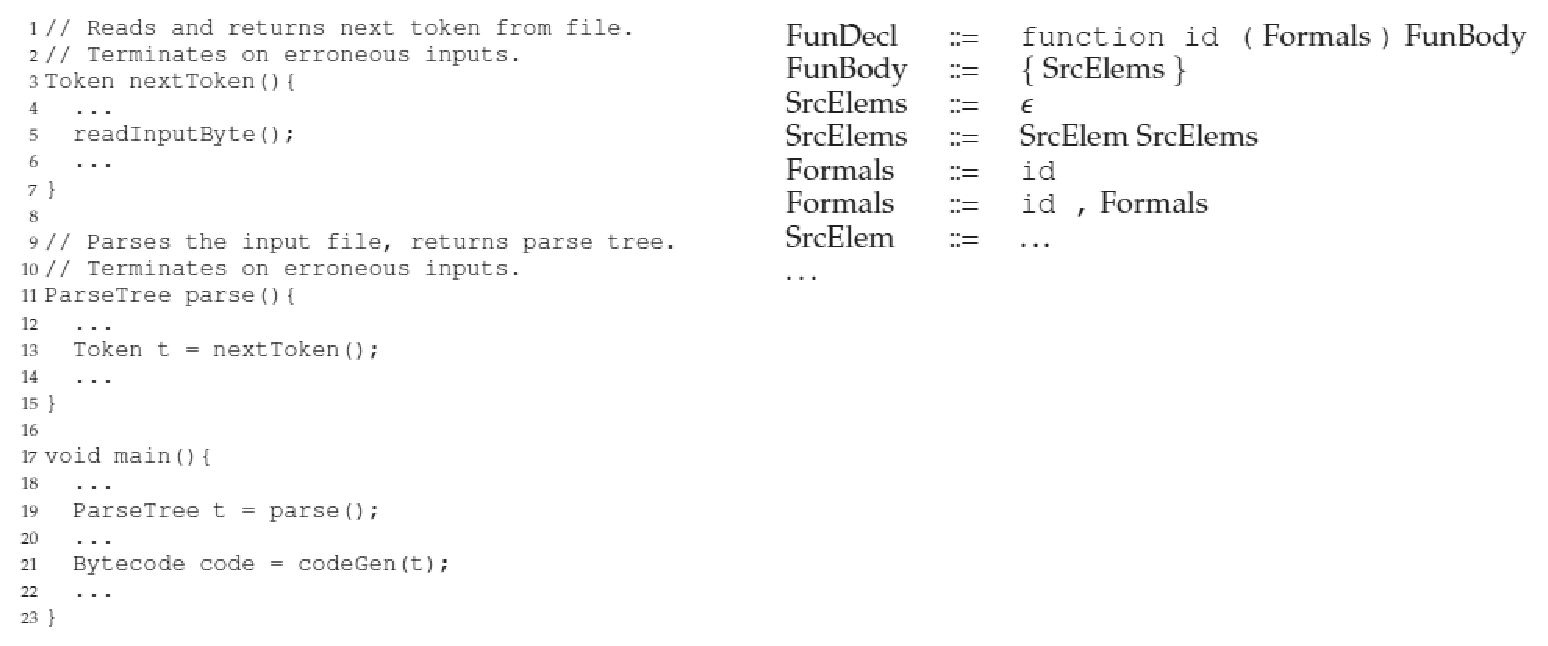
\includegraphics[scale=0.6]{grammar.eps} 
\caption{\label{fig:grammar} Interpreter and fragment of a context-free grammar for JavaScript. }
\end{figure}

%\begin{figure}[h]
%\centering
%\includegraphics[scale=0.6]{interpreter.eps} 
%\caption{\label{fig:interpreter}Sketch of an interpreter. The interpreter processes the inputs in stages: lexer (function nextToken), parser (function parse), and code generator (function codeGen). Next, the interpreter executes the generated bytecode.}
%\end{figure}

Consider the interpreter sketched in Figure \ref{fig:grammar} and the JavaScript grammar partially defined in Figure \ref{fig:grammar}. By tracking the tokens returned by the lexer, i.e., the function nextToken in Figure \ref{fig:grammar}, and considering those as symbolic inputs, their dynamic test generation algorithm generates constraints in terms of such tokens. For instance, running the interpreter on the valid input:

\begin{center}
$function$  $f()$ $\{\}$
\end{center}

This input may correspond to the sequence of symbolic token constraints:

\begin{center}

$token_0 = function$ \\
$token_1 = id$ \\
$token_2 = ($ \\
$token_3 = )$ \\
$token_4 = \{$ \\
$token_5 = \}$

\end{center}


Negating the fourth constraint in this path constraint leads to the new sequence of constraints:
\begin{center}

$token_0 = function$ \\
$token_1 = id$ \\
$token_2 = ($ \\
$token_3 \neq )$ 

\end{center}

There are many ways to satisfy this constraints but most solutions lead to non-parsable inputs. In contrast, our grammar-based constraint solver can directly conclude that the only way to satisfy this constraint while generating a valid input according to the grammar is to set:

\begin{center}

$token_3 = id$ 

\end{center}

and to complete the remainder of the input with, say,

\begin{center}

$token_4 = )$ \\
$token_5 = \{$ \\
$token_6 = \}$ \\


\end{center}

Thus, the generated input that corresponds to this solution is:

\begin{center}
$function$  $f(id)$ $\{\}$
\end{center}

Here id can be any identifier. Similarly, the grammar-based constraint solver can immediately prove that negating the third constraint in the previous path constraint, thus leading to the new path constraint:

\begin{center}

$token_0 = function$ \\
$token_1 = id$ \\
$token_2 \neq ($ 


\end{center}
is unsolvable, i.e., there are no inputs that satisfy this constraint and are recognized by the grammar. Grammar-based
whitebox fuzzing prunes in one iteration the entire subtree of lexer executions corresponding to all possible nonparsable
inputs matching this case.

\subsection{Grammar-based Extension to Whitebox Fuzzing}
Grammar-based whitebox fuzzing is an extension of the algorithm of whitebox fuzzing~\cite{fuzzing}. Their algorithm requires a grammar $G$ that describes valid inputs. Instead of marking the bytes in program inputs as symbolic, grammar-based whitebox fuzzing marks tokens returned from a tokenization function, such as nextToken in Figure \ref{fig:grammar} as symbolic; thus grammar-based whitebox fuzzing associates a symbolic variable with each token, and symbolic execution tracks the influence of the tokens on the control path taken by the program $P$. The algorithm uses the grammar $G$ to require that the new input not only satisfies the alternative path constraint but is also in the language accepted by the grammar. As the examples in the introduction illustrate, this additional requirement gives two advantages to grammar-based
whitebox fuzzing: it allows pruning of the search tree corresponding to invalid inputs (i.e., inputs that are not accepted by the grammar), and it allows the direct completion of satisfiable token constraints into valid inputs.

\subsection{Context-free Constraint Solver}
A context-free constraint solver takes as inputs a context-free grammar $G$ and a regular expression $R$, and returns either a string $s \in L(G) \bigcap L(R)$, or $\bot$ if the intersection is empty. They gives an algorithm to describe an decision procedure for such a constraint solver. They also provide three technical steps to eliminate recursion for the
start symbol $S$: (1) Assign $G$ to $G'$; (2) Duplicate productions for starting nonterminal $S$ by creating $S'$ in $G'$; (3) rename $S$ to $S'$ (but not in the duplicated productions). The algorithm exploits the fact that, by construction, any regular language $R$ always constrains only the first $n$ tokens returned by the tokenization function, where $n$ is the highest index $i$ of a token variable $token_i$ appearing in the constraint represented by $R$. The algorithm starts by converting the path constraint into a regular expression $R$. This is straightforward and involves grouping the constraints in $pc$ by the token variable index. The algorithm employs a simple unroll-and-prune approach: in the $i$th iteration of the main loop, the algorithm unrolls the right-hand sides of productions to expose a $0 \ldots i$ prefix of terminals, and prunes those productions that violate the constraint $c_i$ on the $i$th token variable $token_i$ in the regular expression $R$. During each round of unrolling and pruning, the algorithm uses the worklist $W$ to store productions that have not yet been unrolled and examined for conformance with the regular expression.

After the unrolling and pruning, the algorithm checks emptiness~\cite{theorybook} of the resulting language $L(G')$ and generates a string $s$ from the intersection grammar $G'$. For speed, their implementation uses a bottom-up strategy
that generates a string with the lowest derivation tree for each nonterminal in the grammar, by combining the strings
from the right-hand sides of productions for nonterminals. This strategy is fast due to memorizing strings during generation.

To illustrate the algorithm, they provides an example, a simplified $S$-expression grammar. Starting with the initial
grammar, the algorithm unrolls and prunes productions given a regular path constraint. The grammar is ($S$ is the start
symbol, nonterminals are uppercase).

\begin{center}

$S :=  (let ((id$ $S))$ $S) | (Op$ $S$ $S) | num | id$ \\
$Op := + | −$ 


\end{center}

and the regular path constraint is:

\begin{center}


$token_1 = \{(\}$ \\
$token_2 = \{+\}$ \\
$token_3 = \{(\}$ \\
$token_4 = \{(, ), num, id, let\}$ \\

\end{center}

Before the main iteration, the grammar is:

\begin{center}

$S' :=  (let ((id$ $S'))$ $S') | (Op$ $S'$ $S') | num | id$ \\
$Op := + | −$ \\
$S :=  (let ((id$ $S'))$ $S') | (Op$ $S'$ $S') | num | id$ \\

\end{center}

Next, the main iteration begins. The first conjunct in the grammar constraint is $token_1 \in \{(\}$, therefore the algorithm removes the last two productions from the grammar. The result is the following grammar.

\begin{center}

$S' :=  (let ((id$ $S'))$ $S') | (Op$ $S'$ $S') | num | id$ \\
$Op := + | −$ \\
$S :=  (let ((id$ $S'))$ $S') | (Op$ $S'$ $S') $ \\

\end{center}

In the next iteration of the for loop, the algorithm examines the second conjunct in the regular path constraint,
$token_2 \in \{+\}$. The algorithm prunes the first production rule from $S$ since let does not match $+$, and then expands the nonterminal $Op$ in the production $S := (Op$ $S'$ $S')$. The production is replaced by two productions,
$S := (+$ $S'$ $S')$ and $S := (-$ $S'$ $S')$, which are added to the worklist $W$. The grammar $G'$ is then

\begin{center}

$S' :=  (let ((id$ $S'))$ $S') | (Op$ $S'$ $S') | num | id$ \\
$Op := + | −$ \\
$S := (+$ $S'$ $S') | (-$ $S'$ $S')$ \\

\end{center}

In the next iteration, the second of the new productions is removed from the grammar because it violates the grammar constraint. After the removal, the execution is now again at the top of the iteration.

\begin{center}

$S' :=  (let ((id$ $S'))$ $S') | (Op$ $S'$ $S') | num | id$ \\
$Op := + | −$ \\
$S := (+$ $S'$ $S') $ \\

\end{center}

After 2 more iterations of the for loop, the algorithm arrives at the final grammar:

\begin{center}

$S' :=  (let ((id$ $S'))$ $S') | (Op$ $S'$ $S') | num | id$ \\
$Op := + | −$ \\
$S := (+$ $(let$ $((id$ $S'))$ $S')$ $S')$ \\

\end{center}

As the last two steps, the algorithm checks that $L(G') \neq \emptyset$ , and generates a string $s$ from the final grammar $G'$ for the intersection of $G$ and $R$. Our bottom-up strategy generates the string $S := (+$ $(let$ $((id$ $num))$ $num)$ $num)$ . From this string of tokens, our tool generates a matching string of input bytes by applying an application-specific detokenization function.